%\usepackage{subfig}
\begin{figure}[H]
    \centering
    \subfloat[传统交叉验证]{
        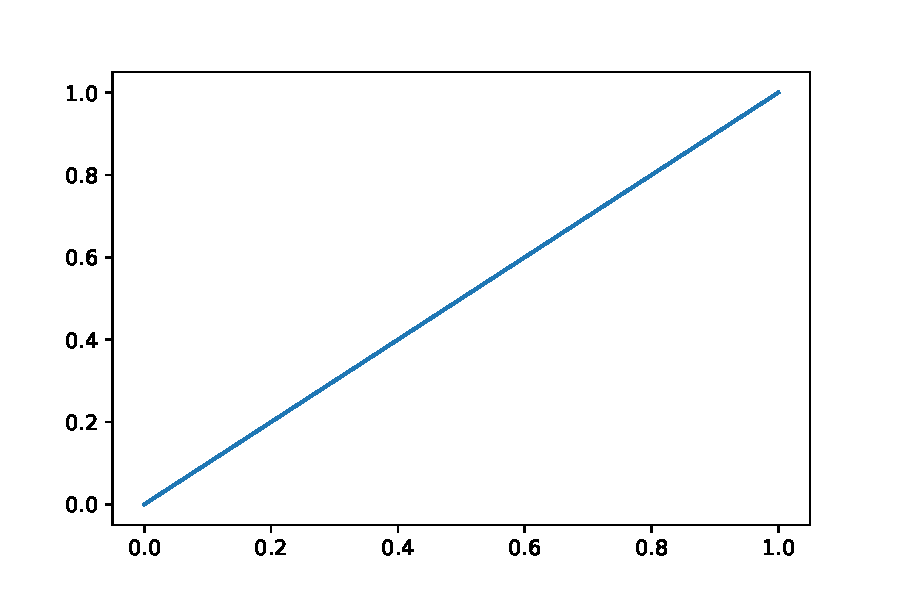
\includegraphics[width=0.48\textwidth]{./asset/figure.pdf}
        \label{fig:cv-传统}}
    \subfloat[时间序列的交叉验证]{
        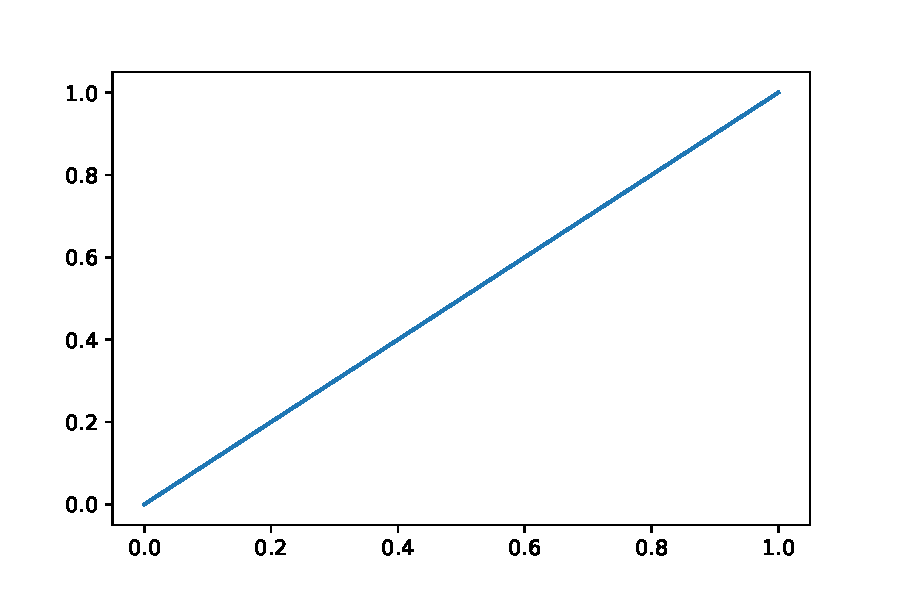
\includegraphics[width=0.48\textwidth]{./asset/figure.pdf}
        \label{fig:cv-时序}}
    \caption{两种交叉验证方式的对比(以五折交叉验证为例)}\label{sub_fig}
  \end{figure}